%%
%% Copyright 2007, 2008, 2009 Elsevier Ltd
%%
%% This file is part of the 'Elsarticle Bundle'.
%% ---------------------------------------------
%%
%% It may be distributed under the conditions of the LaTeX Project Public
%% License, either version 1.2 of this license or (at your option) any
%% later version. The latest version of this license is in
%%  http://www.latex-project.org/lppl.txt
%% and version 1.2 or later is part of all distributions of LaTeX
%% version 1999/12/01 or later.
%%
%% The list of all files belonging to the 'Elsarticle Bundle' is
%% given in the file `manifest.txt'.
%%
\documentclass[5p,authoryear,preprint,12pt]{elsarticle}
\makeatletter\if@twocolumn\PassOptionsToPackage{switch}{lineno}\else\fi\makeatother

\usepackage{multirow,booktabs,setspace,caption}
\usepackage{tabulary,tabularx,siunitx}
\usepackage{amsfonts,amsmath,amssymb}
\usepackage[T1]{fontenc}
%\usepackage{latexmk}
\usepackage[x11names]{xcolor}
\usepackage[colorlinks]{hyperref}
\usepackage{natbib}
\usepackage{pdflscape}
\makeatletter
\let\save@ps@pprintTitle\ps@pprintTitle
\def\ps@pprintTitle{\save@ps@pprintTitle\gdef\@oddfoot{\footnotesize\itshape \null\hfill\today}}
\def\hlinewd#1{%
 \noalign{\ifnum0=`}\fi\hrule \@height #1%
 \futurelet\reserved@a\@xhline}
\def\tbltoprule{\hlinewd{.8pt}\\[-12pt]}
\def\tblbottomrule{\noalign{\vspace*{6pt}}\hline\noalign{\vspace*{2pt}}}
\def\tblmidrule{\noalign{\vspace*{6pt}}\hline\noalign{\vspace*{2pt}}}
\AtBeginDocument{\ifNAT@numbers \biboptions{sort&compress}\fi}
\makeatother

 


\usepackage{ifluatex}
\ifluatex
\usepackage{fontspec}
\defaultfontfeatures{Ligatures=TeX}
\usepackage[]{unicode-math}
\unimathsetup{math-style=TeX}
\else 
\usepackage[utf8]{inputenc}
\fi 
\ifluatex\else\usepackage{stmaryrd}\fi

 
%%%%%%%%%%%%%%%%%%%%%%%%%%%%%%%%%%%%%%%%%%%%%%%%%%%%%%%%%%%%%%%%%%%%%%%%%%
% Following additional macros are required to function some 
% functions which are not available in the class used.
%%%%%%%%%%%%%%%%%%%%%%%%%%%%%%%%%%%%%%%%%%%%%%%%%%%%%%%%%%%%%%%%%%%%%%%%%%
\usepackage{url,multirow,morefloats,floatflt,cancel,tfrupee}
\makeatletter


\AtBeginDocument{\@ifpackageloaded{textcomp}{}{\usepackage{textcomp}}}
\AtBeginDocument{\hypersetup{citecolor=DodgerBlue4}}
\makeatother
\usepackage{colortbl}
\usepackage{xcolor}
\usepackage{pifont}
\usepackage[nointegrals]{wasysym}
\urlstyle{rm}
\makeatletter

%%%For Table column width calculation.
\def\mcWidth#1{\csname TY@F#1\endcsname+\tabcolsep}

%%Hacking center and right align for table
\def\cAlignHack{\rightskip\@flushglue\leftskip\@flushglue\parindent\z@\parfillskip\z@skip}
\def\rAlignHack{\rightskip\z@skip\leftskip\@flushglue \parindent\z@\parfillskip\z@skip}

%Etal definition in references
\@ifundefined{etal}{\def\etal{\textit{et~al}}}{}


%\if@twocolumn\usepackage{dblfloatfix}\fi
\usepackage{ifxetex}
\ifxetex\else\if@twocolumn\@ifpackageloaded{stfloats}{}{\usepackage{dblfloatfix}}\fi\fi
\DeclareMathOperator*{\argmin}{argmin}
\DeclareMathOperator*{\argmax}{argmax}

\AtBeginDocument{
\expandafter\ifx\csname eqalign\endcsname\relax
\def\eqalign#1{\null\vcenter{\def\\{\cr}\openup\jot\m@th
 \ialign{\strut$\displaystyle{##}$\hfil&$\displaystyle{{}##}$\hfil
   \crcr#1\crcr}}\,}
\fi
}

%For fixing hardfail when unicode letters appear inside table with endfloat
\AtBeginDocument{%
 \@ifpackageloaded{endfloat}%
  {\renewcommand\efloat@iwrite[1]{\immediate\expandafter\protected@write\csname efloat@post#1\endcsname{}}}{\newif\ifefloat@tables}%
}%

\def\BreakURLText#1{\@tfor\brk@tempa:=#1\do{\brk@tempa\hskip0pt}}
\let\lt=<
\let\gt=>
\def\processVert{\ifmmode|\else\textbar\fi}
\let\processvert\processVert

\@ifundefined{subparagraph}{
\def\subparagraph{\@startsection{paragraph}{5}{2\parindent}{0ex plus 0.1ex minus 0.1ex}%
{0ex}{\normalfont\small\itshape}}%
}{}

% These are now gobbled, so won't appear in the PDF.
\newcommand\role[1]{\unskip}
\newcommand\aucollab[1]{\unskip}
 
\@ifundefined{tsGraphicsScaleX}{\gdef\tsGraphicsScaleX{1}}{}
\@ifundefined{tsGraphicsScaleY}{\gdef\tsGraphicsScaleY{.9}}{}
% To automatically resize figures to fit inside the text area
\def\checkGraphicsWidth{\ifdim\Gin@nat@width>\linewidth
	\tsGraphicsScaleX\linewidth\else\Gin@nat@width\fi}

\def\checkGraphicsHeight{\ifdim\Gin@nat@height>.9\textheight
	\tsGraphicsScaleY\textheight\else\Gin@nat@height\fi}

\def\fixFloatSize#1{}%\@ifundefined{processdelayedfloats}{\setbox0=\hbox{\includegraphics{#1}}\ifnum\wd0<\columnwidth\relax\renewenvironment{figure*}{\begin{figure}}{\end{figure}}\fi}{}}
\let\ts@includegraphics\includegraphics

\graphicspath{{Figs/}}

\def\inlinegraphic[#1]#2{{\edef\@tempa{#1}\edef\baseline@shift{\ifx\@tempa\@empty0\else#1\fi}\edef\tempZ{\the\numexpr(\numexpr(\baseline@shift*\f@size/100))}\protect\raisebox{\tempZ pt}{\ts@includegraphics{#2}}}}

%\renewcommand{\includegraphics}[1]{\ts@includegraphics[width=\checkGraphicsWidth]{#1}}
\AtBeginDocument{\def\includegraphics{\@ifnextchar[{\ts@includegraphics}{\ts@includegraphics[width=\checkGraphicsWidth,height=\checkGraphicsHeight,keepaspectratio]}}}

\DeclareMathAlphabet{\mathpzc}{OT1}{pzc}{m}{it}

\def\URL#1#2{\@ifundefined{href}{#2}{\href{#1}{#2}}}

%%For url break
\def\UrlOrds{\do\*\do\-\do\~\do\'\do\"\do\-}%
\g@addto@macro{\UrlBreaks}{\UrlOrds}



\edef\fntEncoding{\f@encoding}
\def\EUoneEnc{EU1}
\makeatother
\def\floatpagefraction{0.8} 
\def\dblfloatpagefraction{0.8}
\def\style#1#2{#2}
\def\xxxguillemotleft{\fontencoding{T1}\selectfont\guillemotleft}
\def\xxxguillemotright{\fontencoding{T1}\selectfont\guillemotright}

\newif\ifmultipleabstract\multipleabstractfalse%
\newenvironment{typesetAbstractGroup}{}{}%

%%%%%%%%%%%%%%%%%%%%%%%%%%%%%%%%%%%%%%%%%%%%%%%%%%%%%%%%%%%%%%%%%%%%%%%%%%
\emergencystretch 20pt \tolerance = 1500 \def\floatpagefraction{0.8}




\begin{document}

\begin{frontmatter}
	
\title{AAApplication of Non--Supervised Learning Tools and Visualization Techniques to Understand the Segmentation Dynamics of First--Year Engineering Students
}
  
\author[a]{Patricio Salas}
\ead{patricioasalas@udec.cl}
\author[a]{Rodrigo De la Fuente\corref{cor1}}
\ead{rodelafuente@udec.cl}
\cortext[cor1]{\hspace{0.1cm}Corresponding author}
\author[b]{Andres Riquelme}
\ead{juriquelme@utalca.cl}
%\fi
\address[a]{Department of Industrial Engineering\unskip, 
	Universidad de Concepci\'{o}n\unskip, Concepci\'{o}n\unskip, Chile}
\address[b]{Facultad de Econom\'{\i}a y Negocios\unskip, 
  Universidad de Talca}
 

\begin{abstract}
 Multivariate data visualization techniques are powerful methods for extracting information from large databases. Among these techniques, grouping and projecting data from high--dimensional to low--dimensional spaces play an important role, allowing to discover hidden structures in the data. This work presents a methodology for the segmentation and visualization of academic information of first--year students from the college of engineering at the University of Concepci\'on, Chile. First, we use Kohonen's Self--Organizing Map (SOM) to generate a non--linear projection to a two--dimensional space of the academic records. Then, students' are clustered applying the $k$-means algorithm to the SOM results. Next, we use the Local Interpretable Model-agnostic Explanation (LIME) algorithm to determine the relative contribution of each feature to the centroid of each cluster. After that the clusters are geo--spatially projected to observe patterns among schools and network visualizations are generated to understand the dynamics of how high--schools students flow to the programs offered by the College of Engineering. Finally, using the squarified treemap algorithm, we visualize the participation that different schools have had on enrollment over time. The proposed methodology clearly showed that students coming from the clusters with better academic performance, which correlates with privates schools, prefer degrees in either Chemical, Industrial, Civil, or Mechanical Engineering, while those coming from the worst performing groups composed mainly of public schools, enrolled in Telecommunications, and Materials Science Engineering. Additionally, we observe that subsidized private schools have gained participation in all clusters, becoming a natural replacement for public schools and a serious competitor to private schools.
\end{abstract}
\end{frontmatter}
  

\section{Introduction}

Since the emergence of a global economy, education has played the most crucial role and contributed the greatest to the development of a country. In particular, post-secondary education has become vital for all developed countries to maintain domestic prosperity and promote international competitiveness \citep{ma2013profiles}. With increased enrollment, dropouts become a concern \citep{ma2013profiles}. Dropout is a problem that affects both developed and developing countries. For example, in the USA, several studies have shown that on average, 60\% of students do not complete their undergraduate studies \citep{shapiro2015completing, mcfarland2019condition}. In Europe, the situation is similar; as a consequence, they have defined strategies to decrease this educational indicator \citep{vossensteyn2015dropout}. While in Latin America and the Caribbean, according to \citet{marta2017crossroads} on average, about half of the population aged 25-29 who began higher education at some point did not complete their studies, either because they are still studying or because they dropped out. In Chile, according to the information provided by the \emph{Servicio de Información de Educación Superior} (SIES), on average, the dropout rate in freshmen is 24\%. 

A large body of literature \citep{sanchez2005using, donoso2007analisis, chacon2012analytics, miranda2017analisis} indicate that there is high variability in the factors that motivate the entrance and permanence of students in universities, ranging from economic to academic issues. Consequently, desertion is been addressed more broadly as a problem that generates negative impacts not only at the individual level, but also at institutional, regional, and national levels. Additionally, studies show that desertions occur more significantly during the first year of studies \citep{donoso2007analisis,gonzalez2018estimaciones}. Thereby, educational institutions have started to generate policies and strategies leaning to increase retention of freshmen.

Additionally, \citet{braxton2005theoretical} indicated that academic managers should know their students' characteristics to adopt the most adequate actions for their formative development. Given that the structure and nature of these characteristics have an impact on the students' graduation rate (and/or dropout rate), their profiles can be configured based on three categories of data \citep{gianoutsos2011comparing}: Demographic profile ( gender, socio--economic level, parents' educational level, place of residence, etc.), Academic profile (high school grades, entrance examinations scores, etc.) and Enrollment profile (number of taken or passed credits, undergraduate degree, etc.)

Chile is no stranger to the phenomenon of desertion of freshmen, it is so that in recent decades. Moreover, rapid economic development increased the demand, provoking a sudden rise of institutions offering higher education. This new scenario generated changes that are currently difficult to observe in the students' selection and admission processes. Besides, the increase in coverage and enrollment in higher education has brought significant changes in the socio-economic profile of incoming students. According to data presented in \citet{gallegos2018factores}, in the early 1990s, there were $245,000$ students enrolled in post-secondary education, while by 2017 this number reached a total of $1,162,306$. The study also shows that the higher education system has switched from being for an elite to be for a broader target \citep{gallegos2018factores}. This new reality makes more relevant the study of the factors that explain entry to higher education and the determinants of school dropout \citep{acuna2010access}. For example, \citet{rolando2012retention} showed that sex, high school education quality, and standardized admission test results have a strong influence on the risk of dropping out during the first year. Similarly, \citep{manzi2008estudio} showed that the results obtained in the admission test are good predictors of university success. Regarding engineering students, \citep{diaz2009factores} found that the most relevant factor for dropout is the quality of the preparation obtained during high school.

Summarizing, is imperative to study the phenomenon of desertion in higher education because leaving university without a degree has significant consequences for individuals, institutions, and society \citep{bernardo2017freshmen, sarra2018identifying}. To successfully reduce school dropout, it is essential to understand what the underlying determinants of dropout are and which students are at risk of dropping out of school \citep{berens2018early}. 

To better understand this new scenario we propose the use of ML algorithms which are a competitive alternative to statistical approaches. This article presents a methodological procedure that loosely couples proposes unsupervised learning to organize and then clusterize student data, and visualization techniques to understand the clusters' dynamics from four different view points: 1) Covariate contribution (LIME), 2) Geographic configuration (GIS), 3) Student--major dynamics (Social Networks), and 4) High-schools dynamics (TreeMaps). Figure \ref{methods} illustrates the algorithmic structure of this article.

%In this work, we propose the joint use of different methods of visualization and machine learning (ML). A self-organized map clustering approach is proposed to segment to the freshmen of undergraduate engineering careers at the University of Concepción. Then, this information will be linked to the students' high schools to represent spatial dynamics, to understand the flow dynamics from high--schools to the different academic programs offered by the college of engineering and to understand the temporal evolution of the contribution of students from every one of these, using GIS, social network analysis and squarified treemaps, respectively. Finally, to have a tool to predict which segment a new student belongs to, we adjust a supervised classification model (Random Forest) and to explain the effects of features over the predictions we propose the use of LIME, a technique capable of explaining the predictions of any classifier from an interpretable model locally \citep{ribeiro2016model}. Figure \ref{methods} illustrates the methodology employed in this work.

\begin{figure}[h]
	\centering
	\includegraphics[trim={0cm 0cm 0cm 0cm},clip, scale=1]{methods}
	\caption{Algorithmic structure of the proposed methodology}
	\label{methods} 
\end{figure}

We believe our methodology provides a complete radiography of first-year students dynamics, and these result could be used to develop internal marketing strategies focused on both capturing better students and reducing dropout rate.

The rest of this article is structured as follows: Section 2 presents the literature review. Section 3 describes the methods and data used in the application, followed by the results in Section 4. Next, Section 5 contains a brief discussion of our analysis. Finally, Section 6 closes the paper with concluding remarks.


\section{Literature Review}

%%% Economic perspective

Since the seminal paper by \citet{becker1962}, investment in human capital is modeled as a financial decision. In one hand, high school graduates can enroll in a higher education institution and forgo part of the wage they can make in the job market while studying. On the other hand, they can go full time to the job market. The rationale behind the decision is that after graduation, the increase in earnings can offset the present value of the foregone income. \citet{dillon2017} find that college quality increases earnings ten years after graduation. This setup has been broadly extended. \citet{strayer2002} study a two--staged decision process, in which the school quality affects the college choice, which in turn affect earnings. Each stage has different determinants and motivations. 

Many authors focus on the first stage \citep[e.g,][]{zvoch2006freshman,venegas2019higher}, in which students have to decide which college to apply and enroll, and colleges have to choose the best students using limited information of the students quality, usually from standardized tests. There is a broad consensus that the Standardized Admission Test (\textsc{sat}) are valid predictors of many aspects of student success across academic and applied fields \citep{manski1983,camara2000sat,kuncel2007standardized} and that the correct sorting maximizes the efficiency on a human capital production function \citep{sallee2008}. In Chile, the admission process to universities is governed by the use of SAT, and assume that this mecanism guarantees the permanence of the best students at the university \citep{donoso2007analisis,servicio2014panorama}. \citet{rubio2011desercion} shows that access to funding reduces the likelihood of students dropping out of college. Also, it presents evidence that students from public schools are more likely to drop out than those from subsidized or private schools.
	
The matching process between students and colleges is not an easy task, and it differs among different students and college profiles. From the students perspective, \citet{zemsky1983} examine \textsc{sat} distributions to find market profiles defined by socioeconomic characteristics of the student's families and geographic aspirations of the applicants. \citet{manski1983} find evidence that students weight costs, academic quality, and distance when choosing a college. \citet{hoxby2013} suggest that neighborhood characteristics and high school characteristics correlate with the college choice. From the college perspective, \citep{robert2010} discusses the effect of market approaches to the education system under several setups, such as public--private schools and admission systems. Another literature focuses on simultaneous analysis: \citet{fu2014} proposes a structural equilibrium model where heterogeneous students apply to colleges that choose among them using noisy measurements of the student's ability. \citet{dillon2017} find that the mismatch between college and applicants is driven by student's decisions (enrollment and application) rather than college admission decisions, where the mismatch is defined as the difference between student's cognitive ability and the relative college quality. Using the same definition, in a later study, \citep{dillon2017} find that most informed students undematch less and overmatch more. The consequences of mismatch are multiple, and the economic literature has focused the dropout rates. \citet{dillon2018} find that college quality reduces the dropout rates, whereas \citet{stinebrickner2014} use simulations to find that the 45\% of the dropout in the first two years of college can be explained by what students learn from their academic performance.

%%%%%%%
%Chilean universities assume that the admission process guarantees the permanence of the best students at the university \citep{donoso2007analisis}. This has led to a delay in exploring other factors that could deliver a better understanding of the students' actual performance. One of the few studies is by \citet{gansemer2006institutional}, who followed several strategies to determine the functional relationships between institutional economic efforts and retention rates.

%The training profiles of undergraduate careers constitute the offer made by the institutions; these lead to the personal, social, and professional development of students, which results in proper positioning of the university in the market. 

In universities, marketing approaches allow market segments to be identified among future students, building a conceptual model that goes beyond demographics \citep{angulo2010market}. By understanding the people served by the university, it is possible to develop offers that satisfy the target market \citep{lewison2007student} and the segments that conform it \citep{bloom2005market}. Grouping study subjects into homogeneous clusters is one of the most commonly used techniques for identifying consumer segments \citep{saarenvirta1998mining, davari2019data} because this technique allows study a problem from multidimensional perspective.

\iffalse
It is clear from the existing literature the importance of the matching between the student's abilities and the college programs profiles and the consequences of the mismatch in economic efficiency and earnings. The economic literature has analyzed the matching processes using structural models because of their simplicity and ease of interpretation. The newly available data set cannot be fully exploited using these traditional methods. 
\fi
%%%%

A suitable tool to visualize complex multidimensional data is the \textit{Self--Organizing Map} (SOM) of Kohonen \citep{kohonen1995springer,kohonen1982self}. SOM is a very popular unsupervised neural network model for the analysis of high-dimensional patterns in data mining applications \citep{shieh2012new}. It can project
high-dimensional patterns onto a low-dimensional topology map \citep{shieh2012new}. SOM has been used in several fields, including environmental sustainability, hidrology, innovation, computer vision, credit risk assessment, quality control, and financial situation of companies \citep{mostafa2010clustering,haselbeck2019self, segev2012identification,hajek2014visualising,ortega2016smart, bao2019integration,alkahtani2019decision,chen2013clustering}. In education context, \citet{alias2006student} identify significant patterns of student behavior, \citet{saadatdoost2011application} make knowledge discovery from data of an institute of higher education and \citet{nogales2019competencies} analyze the characteristics of undergraduate students in Psychology.  %,wei2013customer}. 

In the field of market segmentation, SOM can help market managers easily recognize market segments accurately, as well as monitor market responses for each segment \citep{wei2012case}. For example, \citet{vellido1999segmentation} realized a exploratory segmentation of on-line shopping market, \citet{hung2008market} realized market segmentation of multimedia on-demand in Taiwan, \citet{wei2012case} developed a market segmentation of a children’s dental clinic. Moreover, cluster analysis can be used as a complementary tool to determine the functional relationship of all the attributes that characterize individuals and to obtain groupings of different sets of them, based mainly on their spatial proximity. Several studies used cluster analysis to perform segmentation, for example, \citet{park2014segmenting} who segmented consumers into four distinct groups based on their beliefs and motives regarding pro--environmental consumer behavior, \citet{rundle2015using} use cluster analysis to identify segments in the context of physical activity. In the educational field, \citet{angulo2010market} propose a market segmentation approach for higher education based on rational and emotional factors \citet{casidy2018taxonomy} develop a taxonomy of university students based on their orientation to achievement and sensitivity to prestige, \citet{davari2019data} realized a combination of quantitative and qualitative approaches to identify different market segments in the education industry. Finally, good segmentation contributes towards a better understanding of the market and customer demands \citep{zhou2019market}, in this sense, the combined use of SOM and cluster method allows a better understanding of market segmentation \citep[e.g.,][]{bao2019integration}.
 
%The integration of supervised and unsupervised ML methods can be useful to improve the understanding of a problem, various applied investigations have shown the advantage of this practice, such as \citet{malek2018random} analyze the healing time of the pediatric fracture, \citet{nam2015hazard} make a risk classification of coastal pine forests, \citet{wu2016patent} build an automatic patent classification system, \citet{dong2015novel} build a hybrid model to predict solar irradiance, and \citet{bao2019integration} propose a combined strategy of integration of unsupervised learning with supervised learning for credit risk assessment.
  
Another well studied application in higher education through the use of ML methods is the prediction of dropout risk, under the a classification problem context \citep{siri2015predicting,aulck2016predicting,beaulac2019predicting}. The emphasis of these applications is maximize the prediction accuracy, while interpretability is studied simply by performing a graphical analysis, thus establishing a certain degree of importance of each explanatory factor within the prediction. However, \citet{ribeiro2016model} propose LIME, a method capable of explaining locally the predictions of a ML model through simpler and more accessible models. The predictive methods offer an interesting framework for brands trying to understand their customers \citep{doi:10.1057/jors.2014.65}. 

Lastly, evidence indicates that market knowledge obtained from segmentation derived from the application of ML methods is improved through the use of information visualization techniques and algorithms, such as: First, the GIS provides an even more solid basis for consumer segmentation, as well as for the selection and deselection of entire geographical areas \citep{pridmore2017market}. In addition, \citet{quesada2017assessing} proposes that GIS techniques can be employed in different marketing areas of a company. Second, the analysis of social networks makes it possible to understand the dynamics that link individuals within the market, which is a vital support for marketing \citep{webster2004network}. In education context, \citet{shields2013globalization} analyses changes in the international network of student mobility in higher education over ten years (1999-2008), using data provided by the UNESCO Institute for Statistics. \citet{sirer2015currents} analyze student enrollment flows in public schools in Chicago, USA. Finally, hierarchical information it is possible to visualize using treemaps, developed by \citet{shneiderman1992tree}, this representation has been widely used in different applications such as business, the stock market and manufacturing \citep [see,][]{keivanpour2019adapting}, in educational \citet{keivanpour2019adapting} developed an interface that allows online student performance monitoring based on the use of treemaps.

\section{Methods and data}
In this section we describe the methods used in this article to understand the segmentation dynamics of first-year engineering studen	ts. Also, the empirical records and variables used in this work are described.

\subsection{Data}

The University of Concepción, located in the B\'io--B\'io Region, Chile, is the largest university in the southern part of the country having an enrollment of $20.000$ students. This study evaluated data of first--year students who entered the college on engineering between 2005 and 2017 and attended high--schools in the B\'io--B\'io Region (7866 students).

The variables that characterize the students are those that define a student's profile, namely: gender, socio--economic level\footnote{Deduced from the type of high school the student attended.}, distance from his/her high school to the university, scores obtained in the university selection test, number of credits passed in the first year and the undergraduate degree pursued. Categorical variables were coded using \emph{one hot encoding} to facilitate their inclusion in ML models.

\subsection{Segmentation}
\subsubsection{Self Organizing Map (SOM)}

The SOM is an unsupervised ML method for multivariate data analysis. It is considered the non--linear version of Principal Components, and it has been applied to group and explore data in various areas \citep{kohonen2013essentials}. SOM models are associated with regular grid nodes and use competitive learning, in which a set of neurons compete among themselves to activate. Once the \emph{winning neuron} is found, it is set as an anchor to update the networks' weights. The fundamental idea behind SOM is to convert a signal from a multidimensional vector to a lower--dimensional space, generally to a one-- or two--dimensional map. In this paper, we considered the particular type of SOM known as the Kohonen network \citep{kohonen1982self,kohonen2013essentials}, which does not require prior assumptions of the data, more than the proper encoding of categorical variables. This kind of SOM has a \emph{feed--forward} structure with a single computational layer arranged in rows and columns.

To adjust a SOM, first, a set of small random values must be generated and assigned to the connection weights of each input with the nodes of the regular grid. Then, for each input, the neurons calculate a discriminant function that provides the basis for competition. Next, the neuron with the lowest value in the discriminant function is declared the winner. This neuron determines the spatial location of a neighborhood of excited neurons, thus generating the basis for cooperation between neighboring neurons. Finally, new neurons decrease their values of discriminant function through appropriate adjustment of connection weights; therefore, improving the response of the winning neuron to input with similar characteristics.

\subsubsection{SOM Algorithm}\hspace{1cm}

The basic SOM algorithm includes the following steps \citep[see,][]{kohonen1995springer,shieh2012new}:
\begin{itemize}
	\item[1.] Select the parameters that define the map topology. Then, randomly generate the weights of the initialization vector corresponding to each neuron.
	\item[2.] The network is fed with the data under analysis to find the best \emph{matching unit} for each input vector. Each $X$ record includes quantitative values of $n$ attributes:
	\begin{eqnarray}\label{input}
	X=[X_{1},\ldots,X_{n}] \hspace{0.2cm} \in \mathbb{R}^{n}
	\end{eqnarray}
	The initial weight vector of the $i$-th neuron is defined as:
	\begin{eqnarray}\label{weight}
	m_{i}=[m_{i1},\ldots,m_{in}]\hspace{0.2cm} \in \mathbb{R}^{n}
	\end{eqnarray}
	Then, for each input record, the \emph{winning neuron} is the one that satisfied Eq. (\ref{winning})
	%\begin{eqnarray}\label{winning}
	\begin{align}\label{winning}
	c=\arg\min_{i}{d(X,m_{i})} \in \mathbb{R}^{n},
	\end{align}
	%\end{eqnarray}
	where $d(X,m_{i})$ is the Euclidean distance between a register and the weight vector of the $i$-th neuron.
	\item[3.] Update the initial weight vector for each neuron using the Eq. (\ref{update})
	\begin{multline}\label{update}
	m_{i}(t+1)=m_{i}(t)+\alpha(t) \\ h_{ci}(t)[X(t)- m_{i}(t)],
	\end{multline}
	where $0<\alpha<1$ is the learning rate and $h_{ci}(t)$ indicate the neighborhood rate of the $i$-th neuron with the \emph{winning neuron}. This is obtained from the Gaussian function
	\begin{eqnarray}\label{neighborhood}
	h_{ct}=\exp\left(\frac{||r_{c}-r_{i}||^{2}}{2\sigma^{2}(t)}\right).
	\end{eqnarray}
	In the Eq. (\ref{neighborhood}), $\sigma$ is the controller of the function domain and decreases as the training process progresses. In addition, $r_{i}$ and $r_{c}$ are the position of the $i$-th neuron and the \emph{winning neuron} (c) in the grid defined by SOM, respectively.
\end{itemize}

%\begin{algorithm}[htb]
%  \KwData{Inicializar el vector de pesos con valores aleatorios.}
%  \KwResult{how to write algorithm with \LaTeX2e }
%  initialization\;
%  \While{not at end of this document}{
%    read current\;
%    \eIf{understand}{
%      go to next section\;
%      current section becomes this one\;
%    }{
%      go back to the beginning of current section\;
%    }
%}
%  \caption{How to write algorithms}
%\end{algorithm}

\subsubsection{SOM Visualization}\hspace{1cm}

The visualization technique used in this research was introduced by \citet{ultsch1990kohonen}. This technique uses heatmaps to relate the average values of each of the attributes, in the weight vector, to a given color, to display the values in a color spectrum. Another outstanding aspect of heatmaps is that they provide the possibility to evaluate the correlation between numerical attributes. Similar color shades in two different maps indicate the direct correlation of the corresponding attributes. Likewise, the intensity of the difference or similarity of color between the maps can show the correlation rate between two variables in different parts of the space.

In general, to visualize groups, the distance between adjacent neurons is calculated, and the result presented in what is known as \emph{\textsc{u}--matrix}\footnote{Unified distance matrix.}. If the attributes of two parts of the space under analysis are similar, then the distance between the weight vectors of the related neurons is small, indicating that both neurons are in the same group of the space under analysis. However, the use of \textit{clustering algorithms} have proven to be more efficient in the generation of clusters \citep{kohonen2013essentials}.

Finally, the number of nodes that make up the grid is related to the number of observations or inputs available. \citet{vesanto2000clustering} showed empirically that a good rule of thumb for the optimal number of neurons in the SOM is:

\begin{eqnarray}\label{size_som}
S=5\cdot\sqrt{N},
\end{eqnarray}
where $N$ is the number of inputs.

\subsubsection{\emph{$K$--means} Algorithm}

The $k-$means algorithm \citep{macqueen1967some} is a clustering method that generates a partition of the data set into $k$ heterogeneous classes between them and homogeneous classes within them. Here, homogeneity represents the spatial proximity of the vectors of observations based on the Euclidean distance. The process begins with $k$ vectors, randomly selected from the dataset, and used as centroids of the temporary clusters. Then, the algorithm calculates the distances between the centroids and all vectors in the dataset, matching each vector to its nearest centroid. After assigning all data, the computation of the new centroids of each cluster is calculated according to the following criteria

\begin{eqnarray}\label{kmeans}
c_{i}=\frac{1}{m_{i}}\sum\limits_{j=1}^{m}x_{ji},
\end{eqnarray}
where $c_{i}$ is the centroid of the $C_{i}$ conglomerate and $m_{i}$ is the number of instances collected in the $i$-th cluster. 

The performance of the algorithm depends heavily on the number of groups to search, a number that is unknown \textit{a priori}. In this work, we applied the \emph{elbow method} criterion, which is a method that analyzes the percentage of variance explained as a function of the number of clusters \citep{bholowalia2014ebk}. However, other criteria, such as the \emph{silhouette} method, could also be used.

\subsection{Visualization}
\subsubsection{Hierarchical Data Visualization}

An efficient method to organize and visualize elements with hierarchical structure is the \emph{treemap} \citep{johnson1991tree}. Initially designed to display files on a computer disk, this type of graph subdivides a rectangular region into small sub--regions that represent the importance of each part in the hierarchy \citep{marson2010automatic}. The algorithm starts with an outer rectangle, defined as the root. Then, its inner space is filled recursively with rectangles in a hierarchical father/son relationship. Each parent is assigned an area of the root rectangle according to its relative weight. When, the problem recreates itself, and the same procedure is applied to each parent, i.e., subdivided into the necessary number of rectangles to accommodate the children within the area assigned to the parent in the hierarchy.

The algorithm proposed by \citet{johnson1991tree} is known as the standard method and suffers from generating very elongated and thin rectangles that make it difficult to distinguish the importance of the information contained. Several types of trees have been proposed \citep{shneiderman2001ordered, bederson2002ordered, cesarano2016heuristic}. We use the grid treemaps proposed by \citet{bruls2000squarified}, a method that allows comparisons between different groups. It recursively inserts, from one of the vertices of the parent rectangle, rectangles that try to keep the aspect ratio wide/height as close to one as possible. Using this procedure, the area represented by the data approximates a square. Consequently, the area of the square is relative to the importance of the data it represents, which simplifies interpretation and evaluation. 

Treemaps are simple to use because they only require three graphical parameters: the display area, the position within the display area, and the color--coding \citep{tu2007visualizing}. Also, the use of different colors helps to distinguish between different groups and allows to show the relationship between the hierarchical levels of parent/child \citep{tu2007visualizing}. 

%Moreover, \citet{lurie2007visual} explains that aspects such as color and geometry of the visualization help the decision--maker to decode low--level aspects of the data. Thereby, treemaps allow not only global but also detailed data characteristics to be observed. Additionally, \citet{vliegen2006visualizing} indicates that an adequate visualization improves the reasoning process by freeing parts of the cognitive system so that it can perform a larger number of higher--order activities, such as the interpretation of complex interactions between data. They present a detailed analysis of the different configurations of treemaps available and their performance in analyzing large volumes of data by evaluating how they preserve high--level features (as a pie chart or histogram would do) while retaining low--level information.

\subsubsection{Local Interpretable Model--agnostic Explanations (LIME)}

Many of the ML algorithms are considered black-boxes with limited interpretability. To overcome this shortcoming, \citet{ribeiro2016model} proposed Local Interpretable Model-agnostic Explanations (LIME), which is a implementation of local surrogate models. Local surrogate models are interpretable models that are used to explain individual predictions of black-box ML models. Following the definition given by \citet{molnar2019}, the main idea of LIME is quite intuitive and consists in understanding why the machine learning model made a specific prediction. LIME shows what happens when predictions disturbances are added to the data in the ML model. The algorithm generates a new dataset consisting of exchanged samples and the corresponding predictions from the black-box model. In this new dataset, LIME trains an interpretable model, which is weighted by the proximity of the sampled instances to the instance of interest. The interpretable model can be, for example, linear regression or a decision tree. The model learned should be a good approximation of the predictions of the machine learning model locally, but it does not have to be a good approximation globally. This type of precision is also called local fidelity.

Mathematically, local surrogate models with interpretability constraint can be expressed as follows \citep{molnar2019}:

\begin{eqnarray}\label{local_surrogate_models}
explanation(x) = \argmin_{g\in G}L(f, g, \pi_{x})+\Omega(g),
\end{eqnarray}
where the explanation model for sample $x$ is the model $g$ (e.g. decision three) that minimizes loss L (e.g. cross-entropy), which measures how close the explanation is to the prediction of the original model $f$ (e.g. an random forest model), while the model complexity $\Omega(g)$ is kept low (e.g. select more parsimonious models). $G$ is the family of possible explanations, for example all possible classification models. The proximity measure $\pi_{x}$ defines the size of the neighborhood around sample $x$.

In this work, we used the classifier Random Forest (RF) how the interpretable model, this method was developed by \citet{breiman2001random}. RF is a learning method based on the assembly and combination of predictions, that is, it is a strategy that aggregates many predictions to reduce variance and improve the robustness and accuracy of the results \citep{polikar2012ensemble, friedman2001elements}. The use of the random forest for classification is a powerful statistical tool and has an excellent performance \citep{diaz2006gene}. 

\subsubsection{Network Analysis}
Networks analysis in marketing science has so far typically been used to analyze relationships between relatively high-level representations of nodes, such as networks of consumers and firms \citep{kakatkar2019marketing}. The presentation of the relationships in a network diagram allows you to see connections between entities. In particular, the use of networks gave us insight into student flows from high schools to majors.

To build the networks we use the Python programming language and the network analysis software Gephi \citep{bastian2009gephi}.
\subsubsection{Spatial Analysis}
Geographic data visualization tools come under the banner of geographic information systems (GIS), which are systems that allow users to visualize, explore, and annotate visual data \citep{france2019marketing}. In this work, we used GIS to know the spatial distribution of the clusters found by utilizing the SOM and k--means algorithms; this was achieved by associating each student with their respective high school of origin.

Spatial data visualizations were generated using Quantum GIS 2.0.1 \citealp{team2018r}. 
\section{Results}
In this section, we show the empirical results of the application of the proposed methodology to the data set concerning engineering students. We seek to answer the following research questions: 1) Can ML be employed to segment engineering students?. 2) How do project the segmented groups to high school dynamics?.

\subsection{Segmentation}

First, to obtain an arrangement and grouping of the students, a SOM was trained. Also, the training process was carried out considering a toroidal structure, thus ensuring that all nodes in the network have access to their neighboring nodes. 

\begin{figure*}[htb!] 
	\centering
	\includegraphics[trim={0cm 0.8cm 0.5cm 1cm},clip,width=0.95\textwidth]{codes3}
	\caption{Pie chart of numeric variables at node level.}
	\label{piechart}
\end{figure*}

To define the number of nodes, we used \eqref{size_som} obtaining 440 nodes; however, we utilized 400 nodes to reduce information dispersion, which produced a $20\times20$ rectangular grid. Additionally, the processing time was low enough to carry out the study using a laptop, being this one of the main advantages of SOM \citep{kohonen2013essentials}.

The ordering of the information provided by SOM made it possible to group students who share similar characteristics, and on average, each node was made up of $20\hspace{0.1cm}(\pm7)$ students. Figure \ref{piechart} shows, for each node, a normalized visualization of the average values of the some numerical variables under study. We averaged the records of all the students grouped within the respective node. Moreover, proper normalization allows us to see the importance of each variable within the node and how its interaction influences the order obtained. Subsequently, to complement the analysis, the respective heatmaps were constructed on the original scale of the variables, as shown in Figure \ref{heatmap}. 

In the case of the variable associated with the weighted score obtained in the \textsc{sat}, there is a small area with high scores that gradually fades away until there is a transverse area of low values, given by the toroidal structure of the model. On the other hand, the score associated with high school qualifications (\textsc{hsq}) shows a more homogeneous distribution of high scores within the map. 

The variable that captures the number of credits approved in the first year shows a behavior that is quite counter--intuitive, given that in the upper part there is a strip of nodes that groups students who passed very few credits in their first year of college (even though many had good grades in college), while the lower strip shows relatively high average values. 

In terms of correlations, both the \textsc{sat} weighted score and the \textsc{hsq} score correlate with the number of credits passed.

An in--depth analysis of students grouped into nodes with high \textsc{hsq} and a low number of credits approved did not show evident patterns explaining why students with excellent academic performance in high school, had difficulties during their first year.

\begin{figure}[htb!] 
	\centering
	\includegraphics[width=0.4\textwidth]{standAloneSOM_V2.pdf}
	\caption{Heatmap of numerical variables in their original scale. The contours show the composition of the clusters.}
	\label{heatmap}
\end{figure}

% Decir que usamos K-MEANS

Now, using the ordering obtained with the SOM, applying the algorithm $k$--means algorithm \citep{wehrens2007self}, we identify four student clusters. Next, the characterization of each cluster was carried out from the covariates defining the students that compose each cluster. Thus, the partition obtained is a subset of the students' universe \citep{ghosh2008service}. 

Figure \ref{fig2} shows the clusters obtained according to SOM ordering. There is a clear separation, except for some nodes, which is explained by the inherent variability of the data.

\begin{figure}[h]
	\centering
	\includegraphics[trim={1cm 0.5cm 1cm 2.2cm},clip, scale=0.45]{cluster}
	\caption{Clusters identified on the SOM from the $k$--means method}
	\label{fig2} 
\end{figure}

To study the effectiveness of the $k$--means method, an \emph{analysis of variance of a factor} \citep{montgomery2017design} was performed with each numerical variable, and the cluster defined factors. Then, we used Tukey's post hoc test when the ANOVA hypothesis test turned out to be significant. The results allow us to infer that there is strong statistical evidence validating the segmentation obtained (see Table \ref{table2}).

%  \begin{center}  
\begin{table}[tbp]
	\caption{ANOVA results comparing cluster means by $k$--means analysis.}
	\label{table2}
	%    \begin{minipage}[c]{1\linewidth}
	\begin{tabular}{lcc}
		\toprule
		& \multicolumn{2}{c}{Statistics} \\
		&  F--score & P--Value\\
		\midrule
		\textsc{sat} \textsc{hsq}  &  803 & $<0.0001$   \\  
		\textsc{sat}  Languaje  & 1598  &$<0.0001$\\
		\textsc{sat}  Mathematics  &2510  &  $<0.0001$  \\
		\textsc{sat}  Science  &  2496  &  $<0.0001$    \\
		\textsc{sat}  Weighted  & 4678  &  $<0.0001$  \\
		Credits Approved  & 1035  &  $<0.0001$  \\
		Distance  &  10.9  &  $0.0001$  \\    
		\bottomrule
	\end{tabular}
	%  \small\textit{Note}. * Hay dos pares de conglomerados cuyas medias no difieren.
	%    \end{minipage}
\end{table}
%  \end{center}

Considering the descriptive analysis at the cluster level given in Table \ref{table1} (see, Appendix), the heatmaps in Figure \ref{heatmap} and the results presented in the Table \ref{table2}, we proceeded to specify the four clusters obtained, which is detailed below:

\begin{figure*}[htb]
	\centering
	\includegraphics[clip,trim={0.1cm 0.5cm 0.3cm 0.2cm},width=15cm,height=12cm]{LIME1}
	\caption{Visual output of LIME for interpretation of predictions made with RF method.}
	\label{fig3}
\end{figure*}

\begin{itemize}
	\item Cluster 1 (Green): This conglomerate contains $17.3\%$ of the total number of students considered in this study. The distribution within the conglomerate according to attended high--school type indicates that $46.6\%$ corresponds to students from private schools, $45.5\%$ to students from subsidized schools and only $7.96\%$ to students who graduated from state--dependent schools. The average distance from schools to the university was $35.1$ \si{\km}. ($40.9 $\si{km}). The students who belong to this cluster, on average, have a weighted college selection test score of 725 ($32.3$), high--school grades score of 724 ($52.8$), and in their first year of college, these students, on average, pass $30.4$ ($8.8$) credits. The undergraduate majors with more representativeness in the conglomerate are Chemical Engineering ($28.5\%$), Industrial Engineering ($17.9\%$) and Civil Engineering ($16.2\%$).
	\vspace{0.5cm}
	\item Cluster 2 (Yellow): In terms of the number of students, this conglomerate is the largest and represents $47.2\%$ of the population under study. Concerning high--school precedence, $22.8\%$ comes from private schools, $51.7\%$ comes from subsidized schools, and the remaining $25.5\%$ corresponds to students from state schools. The average levels of the numerical variables are similar to the values in cluster 1. Additionally, the weighted score in the university selection test was 670 ($28.7$), the score of the high school grades was 680 ($59.9$), and in their first year, these students pass an average of $22.2$ ($12.7$) credits. The majors with the most students from this conglomerate are Industrial Engineering ($14.6\%$), Metallurgical Engineering ($11.6\%$), Civil Engineering ($10.3\%$) and Mechanical Engineering ($10.1\%$).
	\vspace{0.5cm}
	\item Cluster 3 (Orange): A $23.1\%$ of the students are grouped in this cluster, from which $19.9\%$ are students from private schools, $64.8\%$ graduated from subsidized schools and the other $15.3\%$ from state schools. It is striking that this conglomerate concentrates students whose high--schools are closer to the university; with an average distance of $14.6$\si{\km}. ($25.3$\si{km}). In this conglomerate, the average levels of the numerical variables have a significant decrease; thus, the weighted score in the university selection test was 623 ($25.0 $) points, the score of high school grades was 621 ($68.8 $) points and in the first year of college, these students, on average, pass $10.5 $ ($12.1 $) credits. The largest number of students are in the following programs: Civil Engineering -- Common Plan ($23.4\%$), Biomedical Engineering ($12.4\%$), Telecommunications Engineering ($12.0\%$) and Materials Science Engineering ($11.6\%$).
	\vspace{0.5cm}
	\item Cluster 4 (Red): This cluster concentrates $12.4\%$ of the students, being the least numerous. The distribution of students, according to their high--schools, is dominated by those who graduated from state schools ($49.6\%$), followed by students from subsidized schools ($41.3\%)$, while only $9.0\%$ come from private schools. In terms of averages, the grade point average is 645 ($68.7$), the math test scores 606 ($33.0$), the weighted college selection test scores 606 ($31.5$) and the number of credits passed does not exceed 3 ($6.0$). In general, the decrease in performance is considerable, and this conglomerate contains the students whose high--school is geographically far from the University of Concepción. This indicator is, on average, $45.4$\si{\km}. ($41.4$\si{km}).
\end{itemize}

\begin{figure*}[htb]
	\centering
	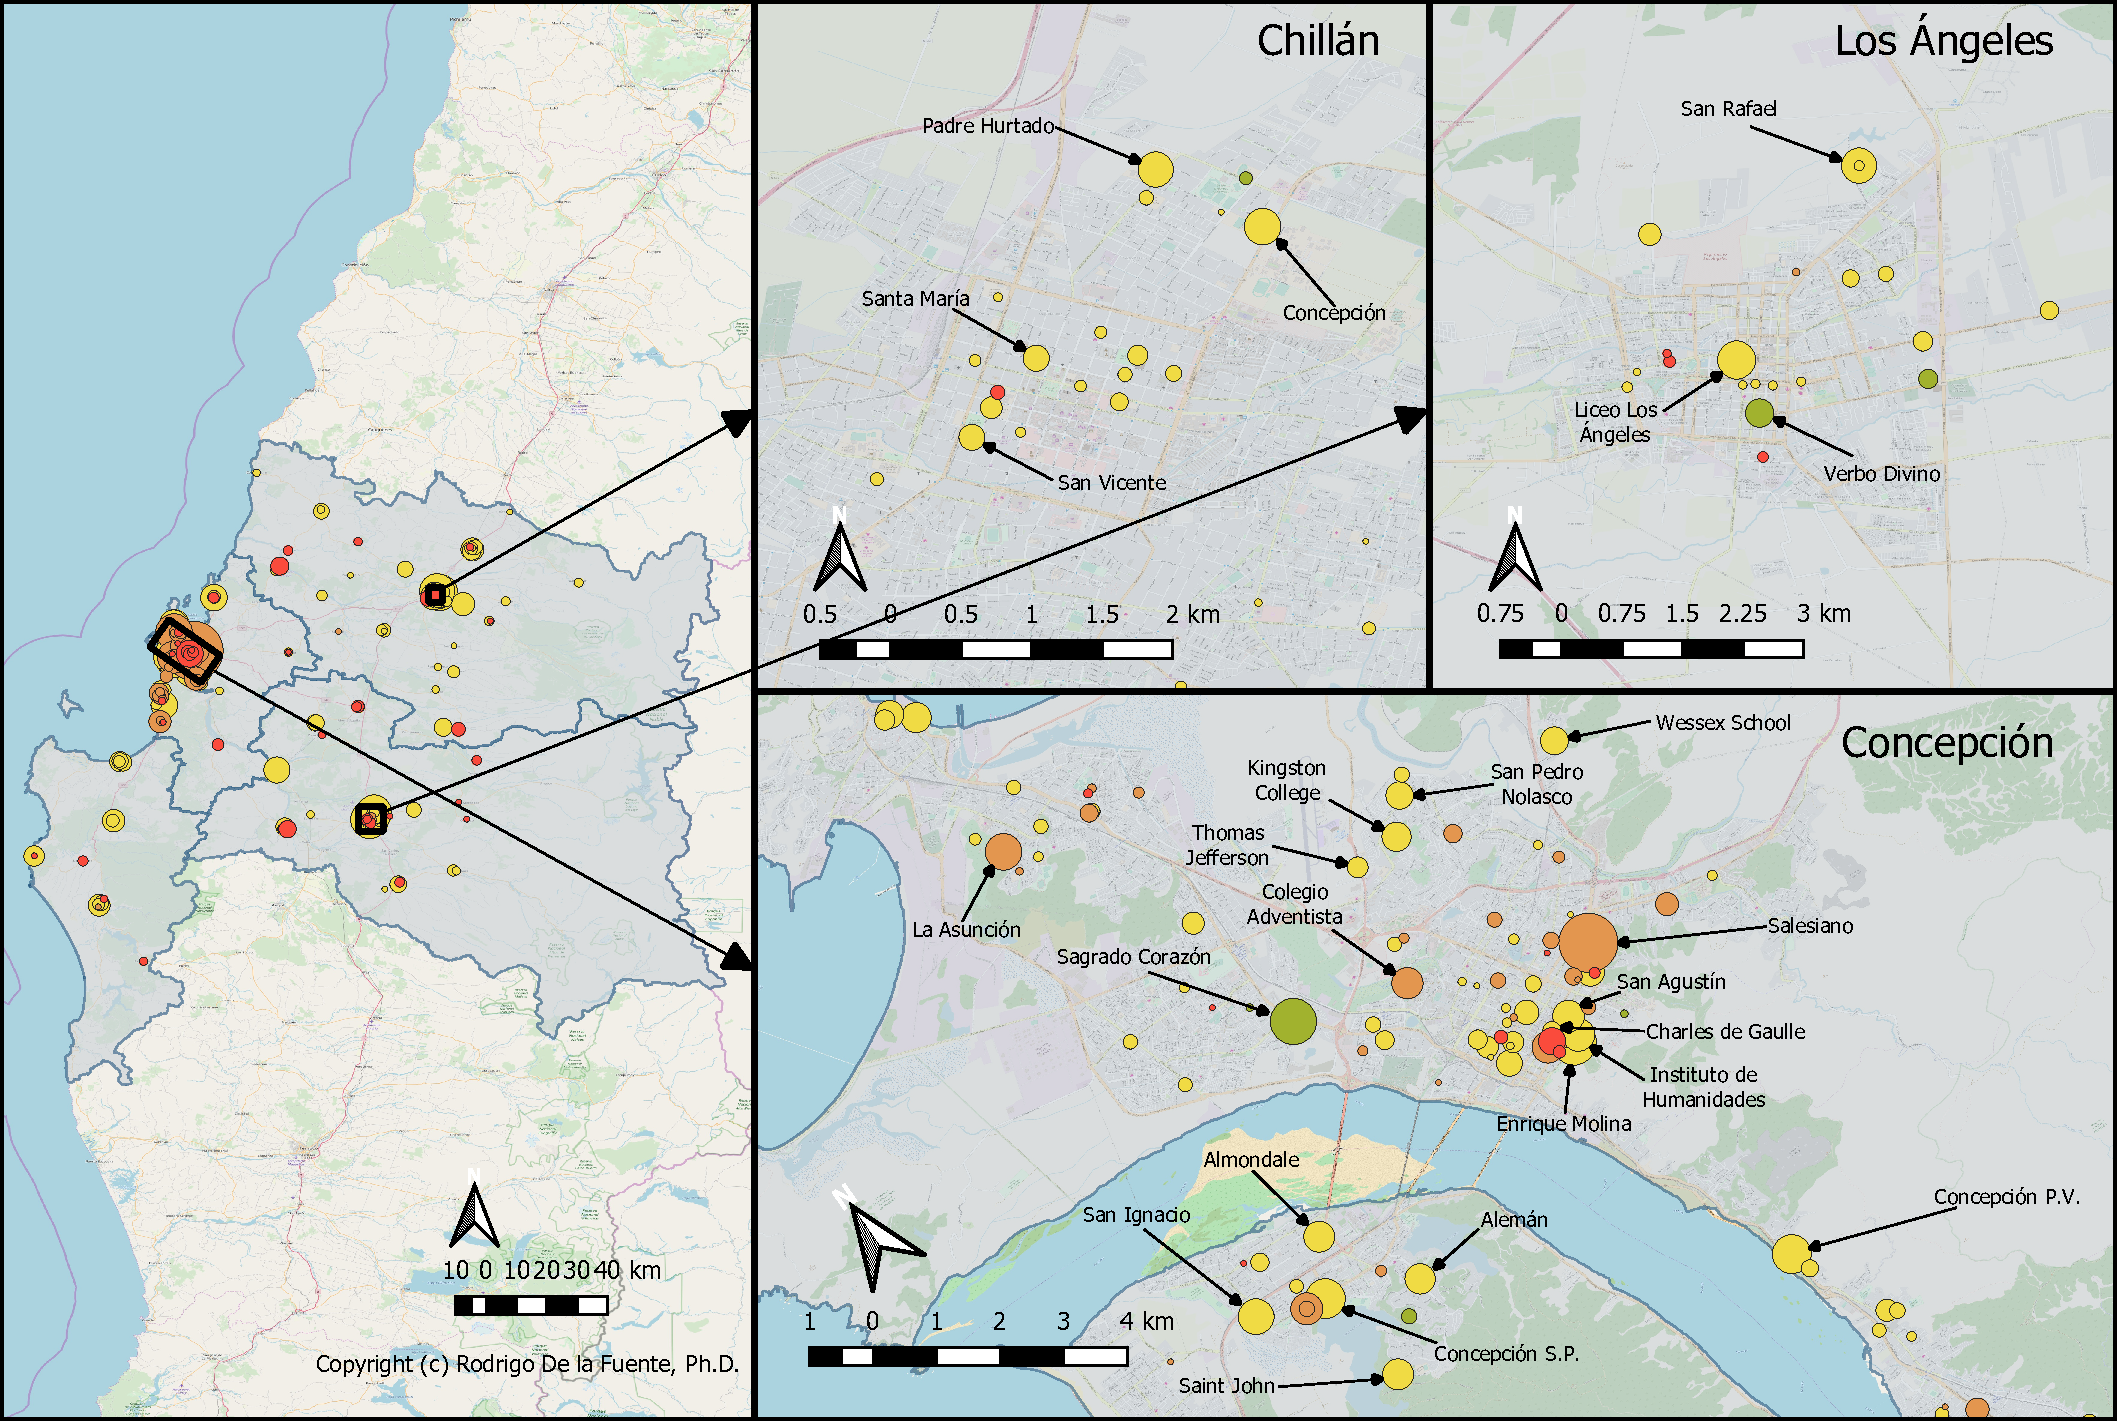
\includegraphics[clip,trim={0cm 0cm 0cm 0cm},width=0.75
	\textheight]{MapaIngUdeC}
	\caption{The spatial composition of high--schools indexed by clusters. B\'io--B\'io Region (left panel), city of Chillán (upper central panel), city of Los Ángeles (upper right panel) and city of Concepción (lower right panel).}
	\label{map}
\end{figure*}

%
% Desde acá comienza la discusión de los resultados o análisis que se pueden realizar a partir del ordenamiento de las observaciones obtenido por el SOM y el posterior agrupamiento realizado mediante el método de clustering k-means
\subsection{Clusters' Dynamics}

The combination of SOM and $k$--means allowed the students to be segmented. With this result, we analyzed different angles of cluster dynamics. First, to classify a new student in a group, a RF was trained, and with LIME, we analyzed the contribution of predictor variables in the prediction. Then we georeferenced the students according to the school of origin.  Next, we analyze the flow of students from schools to careers through social networks. Finally, using the squarified treemap algorithm, we visualize the contribution of different schools in enrollment over time.  

\subsection{Attributes Contribution}
MENCIONAR LOS INDIVIDUOS FICTICIOS QUE SE CREARON

We used LIME to complement the multivariate interpretation of the clusters based on the average values of predictor variables of students that compose each cluster. While the interactions between characteristics are mostly ignored in this way, the visualization casts some light on the black box that is the classifier \citep{amrit2017identifying}. First, using \emph{cross validation}, a RF model with an $82.2\%$ accuracy was obtained; this means, the probability that a student will be well classified in the correct cluster is high. 

Figure \ref{fig3} shows the visual production obtained by LIME; in this figure, we can see that, there is a high probability of correctly classifying a new observation. The main characteristics influencing the prediction are ordered according to their contribution, including the direction of the influence.  We can interpret this as the contribution of the attributes to the result \citep{amrit2017identifying}. Now, for the average student of the first and second groups, high scores in the university selection tests favor or support classification, with the difference that dependence on the middle school is more important in the first case. For the average student in the rest of the groups, the prediction is mainly based on low values in the selection tests and the small number of credits passed in the first year of university. Additionally, in the third group, the distance from high school to university is a factor that contradicts the prediction, which could be explained by the high variability of this variable within the group.

\subsubsection{Georeferencing}

REESCRIBIR ESTE PARRAFO DEMASIADO WE USED

Information from the students' cluster was assigned to each high--school to highlight its geographical disposition and characterization. We used a simple majority vote rule, based on the students' assigned cluster, to match schools to a cluster. Initially, only the name of the schools was available; for this reason, the inverse georeferencing methodology was used to obtain the geographic coordinates of these institutions. 

Figure \ref{map}, displays a map showing the schools. The size of each marker depends on the total number of students coming from the school, and color represents the cluster assigned to each of them. We focus on the most densely populated areas in the Bío--Bío Region. The data presented in each panel (from left to right) of Figure \ref{map} are as follows: In the left panel, a general overview of the whole region is given. On the right panel, schools of the city of Chill\'an are shown, and in the upper right corner, schools located in the city of Los Angeles are displayed. Finally, in the lower right corner panel, schools of the Concepción metro area are represented.

\begin{figure}[htb!] 
	\centering
	\includegraphics[width=0.45\textwidth]{standalone_network}
	\caption{Networking between schools and careers: Clusters 1 and 2 (top), Clusters 3 and 4 (bottom)}
	\label{network}
\end{figure}

From Figure \ref{map}, it can be inferred that, in general terms, there is a broad domain of schools that were assigned to conglomerate C2. In the city of Chillán, few schools fall into conglomerate C3 or C4, and similar behavior can be observed for Los Angeles. On the contrary, in the municipality of Concepción, there is more considerable variability in the classification of schools, which could indicate that perhaps in the latter case the distance from the graduating school to the University of Concepción is not a determining factor of academic performance, or that low--performance students from Chill\'an and Los Angeles have chances of entering the college of engineering than their Concepc\'on counterparts due to other non--observed variables, such as, house--hold income, high--school focus, to name some.

\subsubsection{Social Network}
DESCRIBIR TABLAS DEL APENDICE, NO BASTA CON MENCIONAR QUE ESTÁN

High schools and engineering majors are intrinsically linked as students flow from schools to the various study programs offered by the college of engineering. We defined two large clusters to observe student flow patterns; these clusters arose from the clustering of C1 with C2 and C3 with C4. Thus, Figure \ref{network} show the networks that describe the connections between high schools and majors. The size of the nodes reflects the actual number of students per node in each group, whereas the thickness of the line indicates the number of students that flows from each school. Also, the color of the nodes identifies the type of school: private (pink), subsidized (light blue), and public (green). 

Table \ref{table3} (see, Appendix) summarises the distribution of students, at the school level, who are classified within each cluster. Also, in the first column are the identifiers assigned to each school in Figure \ref{network}.

The upper panel of Figure \ref{network} shows that Industrial, Civil, Chemical, Mechanical, and Metallurgical Engineering are fed mainly by students coming from subsidized and private schools. Also, in the composition of schools, private schools dominate in size, while subsidized schools dominate in quantity. Finally, public schools are under--represented in this conglomerate. 

Likewise, the bottom panel of Figure \ref{network} shows that the conglomerate formed by C3 and C4 is mainly of students from subsidized and public schools. There is an inverse effect to that described in the previous paragraph, with a higher flow towards the following majors: Common Plan, Telecommunications, Materials, Biomedical, and Computer Engineering. As for the composition of the type of school, there is a vast domain of subsidized schools, followed by public schools and little participation of students from private schools. 

\subsubsection{Enrollment Over Time}

Unfortunately, in Figure \ref{network}, it is not possible to appreciate an obvious ordering of schools, and it is even more different to see some temporary behavior of how each type of high education system has evolved through times to majors. To address this problem, we fitted squarified treemaps, ranked by type of high school and maintaining the two conglomerates mentioned above. In addition, to observe temporary effects on the relative contribution of schools, the number of students was divided according to enrollment cohort ($\left[2005,2009\right]$, $\left[2010,2013\right]$ and $\left[2014,2017\right]$).

The treemaps in Figure \ref{treemap} capture the temporary effect of students' enrollment from all types of schools. The top row shows that the contribution of students from public schools has been declining in the best clusters. On the other hand, from the lower row, it can be seen that students from private schools have gradually decreased their participation in conglomerates C3 and C4, similar to what happens with students from public schools. We can see that there is clear evidence of the decline of public education, which coincides with the finding of \citep{paredes2009fin}. Finally, we noted that subsidized schools had gained ground in both clusters.

%\section{Discussion}

\section{Conclusions}
REVISAR LA CITA DE DILLON (ES 2017 o 2018)
Our findings are consistent with the results found by \citep{sallee2008} for the school's side of the system: the more schools, the less polarization, and better segmentation. The identification of four different clusters of applicants aligns nicely with the variety of engineering majors provided by Universidad de Concepci\'on. This variety of careers allows applicants to select majors that better match their abilities. This statement is limited in by two facts: first, the straight interpretation of the results requires that students have full information about the University and programs characteristics. Under this assumption, \citet{dillon2018} propose that families make the college choice based on the applicant ability and their financial constraints. Second, we only have data from Universidad de Concepci\'on, and our results do not necessarily have external validity. This fact is noteworthy if we consider that there are $102$ Engineering and Technology tracks in Chile\footnote{https://www.educaedu-chile.com/carreras-universitarias/ingenieria}) and five Universities offering Civil Engineer in Concepci\'on.\footnote{Universidad de Concepci\'on, Universidad Cat\'olica de la Sant\'isisma Concepci\'on, Universidad del B\'ioB\'io, Universidad de las Am\'ericas, Universidad San Sebasti\'an.}

The contribution of this paper is to extend the study of the students and university programs matching using unsupervised learning methods. These methods exchange interpretability by prediction accuracy. Given the fact that the causes of the mismatch between students and programs are broadly documented, the increase in accuracy and the identification of student profiles is a novel and significant contribution.

Beyond the visual aid provided by the construction of maps, it was possible to directly correlate student information through visualizations, creating a complete learning experience aligned with the objectives and needs of the organization. 

The combination of SOM with the clustering algorithm allowed the identification of four student segments, allowing us to characterized them through the application of visualization tools.

The variables considered the results obtained in the specific university selection tests (Science, Mathematics, and Language), allowing for better discrimination among the different conglomerates. This seems to indicate that students with an excellent academic performance before entering the university have developed better study methods, specific discipline, and individual responsibility, characteristics valued in the Chilean university system.  

This work provides complete radiography of the evolution of the type of students that enter the different majors offered by the college of engineering at the University of Concepci\'on. Geographically speaking, we identified the sectors where they came from and associated their high schools with the characterization of the students that enter each academic program.

The academic information was used to understand the dynamics of segmentation of first--year engineering student at the Universidad de Concepción. Student characteristics at the segment level could be identified, and service strategies can be designed and adapted based on an assessment of these needs.

From this work, the College of Engineering of the University of Concepci\'on will be able to carry out marketing campaigns to attract better students and to improve its current retention levels by providing better information sets to the applicants \citep{chingos2012}.

%%%%%%%%%%%%%%%%%%%%%%%
\section{Acknowledgements}
The authors are grateful to the University of Concepción for providing the data set that allowed this work to be developed. Andr\'es Riquelme acknowledges support from \textsc{Fondecyt} through grant 11160948.

\begin{landscape}
	\begin{figure}
		\includegraphics[trim={0cm 0cm 0cm 0cm},clip,scale=0.42]{treemap_VF2}
		\caption{Treemaps of the number of students per school that fall within the defined clusters.}
		\label{treemap}
	\end{figure}
\end{landscape}	

\bibliographystyle{apa}
\bibliography{referencesV2}

\newpage
\onecolumn
\section*{Appendix}	
\setcounter{table}{0}
\begin{table}[htb]
	\caption{Descriptive summary of variables studied, at cluster level.}
	\label{table1}
	\scalebox{0.9}{%
		\begin{tabular}{lcccc}
			\toprule
			& \multicolumn{4}{c}{Cluster} \\
			& 1 ($n=1332$) & 2 ($n=3631$) & 3 ($n=1773$) & 4 ($n=1130$)\\
			\midrule
			Variable ($\overline{X}\pm \textsc{s.d.}$) & \multicolumn{4}{c}{} \\
			\multicolumn{5}{c}{}\\
			\textsc{hsq}	&	724	(52.8) & 680	(59.9)	&	621	(68.8)	&	645	(68.7)	\\	
			\textsc{sat}	Language	&	691	(51.7)	&	625	(51.1)	&	586	(50.5)	&	561	(54.0)\\
			\textsc{sat}	Mathematics	&	738	(53.2)	&	678	(40.7)	&	642	(33.5)	&	606	(33.0)\\
			\textsc{sat}	Science	&	691	(46.9)	&	635	(40.7)	&	590	(42.8)	&	554	(45.7)\\
			\textsc{sat}	Weigthed	&	725	(32.3)	&	670	(28.7)	&	623	(24)	&	606	(31.5)\\
			Credits Approved	&	30.4	(8.8)	&	22.2	(12.7)	&	10.5	(12.1)	&	2.9	(6.0)\\
			Distance (\si{\km})	&	35.1 (40.9)	&	37.5	(40.4)	&	14.6	(25.3)	&	45.4	(41.4)\\		
			\multicolumn{5}{c}{}\\
			Sex ($Frequency\hspace{0.1cm}(\%)$) & \multicolumn{4}{c}{} \\
			Female & 381 (28.6\%) & 714 (19.7\%) & 331 (18.7\%) & 305 (27.0\%)\\
			Male & 951 (71.4) & 2917 (80.3\%) & 1442 (81.3) & 825 (73.0\%)\\ 
			\multicolumn{5}{c}{}\\
			\multicolumn{5}{l}{High school graduation dependency ($Frequency\hspace{0.1cm}(\%)$)} \\
			Private ($n=1903$) & 620 (46.6\%) & 828 (22.8\%) & 353 (19.91\%) & 102 (9.1\%)\\
			Subsidized ($n=4099$) & 606 (45.5\%) & 1877 (19.9\%) & 1149 (64.81\%) & 467 (41.3\%) \\ 
			Public ($n=1864$) & 106 (7.96\%) & 926 (25.5\%) & 271 (15.3\%) & 561 (49.6\%)\\ 
			\multicolumn{5}{c}{}\\
			\multicolumn{5}{l}{Undergraduate Career ($Frequency$)} \\
			Civil Engineering & 216 & 374 & 10 &  4 \\ 
			Civil Engineering -- Common Plan & 11 & 244 & 414 & 341 \\ 
			Aerospace Engineering & 36 & 92 & 31 & 17 \\ 
			Biomedical Engineering & 76 & 286 & 219 & 70 \\ 
			Materials Science Engineering &  2 & 91 & 205 & 185 \\ 
			Mining Engineering & 40 & 185 & 19 & 19 \\ 
			Electrical Engineering & 32 & 260 & 140 & 48 \\ 
			Electronic Engineering & 65 & 284 & 170 & 29 \\ 
			Telecommunications Engineering &  8 & 53 & 212 & 263 \\ 
			Industrial Engineering & 239 & 529 & 15 & 12 \\ 
			Informatics Engineering & 44 & 248 & 180 & 91 \\ 
			Mechanical Engineering & 127 & 366 & 33 & 17 \\ 
			Metallurgical Engineering & 57 & 420 & 105 & 32 \\ 
			Chemical Engineering & 379 & 199 & 20 &  2 \\ 
			\bottomrule
		\end{tabular}
	}
\end{table}



\begin{table}[htb]
	\footnotesize
	\caption{Distribution of students by cluster in the 50 schools with the highest number of students contributed between 2005 and 2017.}
	\label{table3}
	\centering
	\scalebox{0.9}{%
		\begin{tabularx}{\textwidth}{>{\hsize=0.1\hsize}X>{\hsize=2\hsize}X>{\hsize=1.1\hsize}X>{\hsize=.3\hsize}X>{\hsize=.3\hsize}X>{\hsize=.3\hsize}X>{\hsize=.3\hsize}X>{\hsize=.3\hsize}X}
			\toprule
			\multicolumn{3}{c}{} & \multicolumn{4}{c}{Cluster}& \\
			\cmidrule(lr){4-7}
			\multicolumn{1}{c}{Id} & \multicolumn{1}{c}{School} & \multicolumn{1}{c}{High School Dependency} & C1 & C2 & C3 & C4 & Total \\ 
			\hline
			1 & Colegio Salesiano De Concepcion & Subsidised & 48 & 124 & 202 & 46 & 420 \\ 
			2 & Sagrados Corazones & Private & 119 & 95 & 41 &  6 & 261 \\ 
			3 & Liceo Enrique Molina Garmendia & Public & 11 & 134 & 62 & 42 & 249 \\ 
			4 & Colegio Concepcion San Pedro & Private & 53 & 87 & 48 &  6 & 194 \\ 
			5 & Colegio Concepcion Pedro De Valdivia & Private & 49 & 78 & 43 & 15 & 185 \\ 
			6 & Liceo Los Angeles & Public & 22 & 104 & 10 & 40 & 176 \\ 
			7 & Colegio Concepcion De Chillan & Subsidised & 33 & 101 & 14 & 14 & 162 \\ 
			8 & Liceo La Asuncion Talcahuano & Subsidised & 12 & 67 & 69 & 14 & 162 \\ 
			9 & Colegio San Ignacio Concepcion & Subsidised & 25 & 74 & 51 &  5 & 155 \\ 
			10 & Colegio San Rafael Arcangel Los Angeles & Subsidised & 26 & 90 &  8 & 26 & 150 \\ 
			11 & Colegio Seminario Padre Alberto Hurtado Chillan & Subsidised & 44 & 70 & 18 & 18 & 150 \\ 
			12 & Charles De Gaulle & Private & 52 & 58 & 18 &  3 & 131 \\ 
			13 & Instituto De Humanidades Alfredo Silva S & Private & 36 & 61 & 27 &  6 & 130 \\ 
			14 & Liceo Mauricio Hochschild San Pedro De La Paz & Subsidised &  3 & 33 & 57 & 30 & 123 \\ 
			15 & Liceo De Niñas Concepcion & Public &  6 & 35 & 49 & 29 & 119 \\ 
			16 & Liceo San Agustin De Concepcion & Subsidised & 24 & 47 & 42 &  6 & 119 \\ 
			17 & Colegio Adventista De Concepcion & Subsidised & 10 & 40 & 58 &  8 & 116 \\ 
			18 & Saint Johns School Concepcion & Private & 30 & 69 & 12 &  3 & 114 \\ 
			19 & Colegio Almondale San Pedro De La Paz & Subsidised & 22 & 66 & 22 &  3 & 113 \\ 
			20 & Colegio Aleman De Concepcion & Private & 45 & 46 & 13 &  4 & 108 \\ 
			21 & Liceo Almirante Pedro Espina Ritchie Talcahuano & Public &  5 & 48 & 25 & 29 & 107 \\ 
			22 & Kingston College Concepcion & Private & 25 & 42 & 23 & 10 & 100 \\ 
			23 & Liceo Aleman Del Verbo Divino Los Angeles & Private & 40 & 33 & 16 &  4 & 93 \\ 
			24 & Colegio Etchegoyen Talcahuano & Subsidised & 14 & 41 & 32 &  4 & 91 \\ 
			25 & Colegio Bicentenario Republica Del Brasil & Public &  6 & 50 & 19 & 15 & 90 \\ 
			26 & The Wessex School Concepcion & Private & 26 & 48 & 13 &  3 & 90 \\ 
			27 & Colegio San Pedro Nolasco & Private & 13 & 35 & 27 & 12 & 87 \\ 
			28 & Liceo Comercial Enrique Oyarzun Mondaca & Public &  0 & 26 & 22 & 37 & 85 \\ 
			29 & Liceo Coronel Antonio Salamanca & Public &  4 & 49 &  6 & 22 & 81 \\ 
			30 & Liceo Vicente Alberto Palacios Valdes & Public &  6 & 45 &  8 & 22 & 81 \\ 
			31 & Instituto Santa Maria Chillan & Subsidised & 29 & 38 &  6 &  5 & 78 \\ 
			32 & Liceo Politecnico Heroes De La Concepcion Laja & Public &  4 & 52 &  0 & 22 & 78 \\ 
			33 & Colegio Carmela Romero De Espinosa & Subsidised & 17 & 38 & 21 &  1 & 77 \\ 
			34 & Colegio San Vicente De Paul Chillan & Subsidised & 15 & 46 &  4 & 12 & 77 \\ 
			35 & Colegio Metodista Concepcion & Subsidised & 12 & 29 & 24 &  2 & 67 \\ 
			36 & Colegio Adventista De Chile & Subsidised & 10 & 27 &  7 & 16 & 60 \\ 
			37 & Colegio Aurora De Chile Chiguayante & Subsidised &  4 & 24 & 29 &  3 & 60 \\ 
			38 & Colegio Creacion Concepcion & Subsidised &  5 & 23 & 25 &  6 & 59 \\ 
			39 & Instituto Santa Maria De San Carlos & Subsidised & 13 & 33 &  7 &  5 & 58 \\ 
			40 & Liceo Polivalente Mariano Latorre & Public &  5 & 36 &  1 & 14 & 56 \\ 
			41 & Colegio Teresiano Los Angeles & Subsidised & 16 & 27 &  2 & 10 & 55 \\ 
			42 & Arturo Prat Chacon & Private & 11 & 31 & 10 &  2 & 54 \\ 
			43 & Colegio Concepcion Chiguayante & Subsidised &  6 & 31 & 12 &  5 & 54 \\ 
			44 & Colegio Padre Manuel Dalzon & Subsidised &  3 & 18 & 27 &  6 & 54 \\ 
			45 & Liceo Gabriela Mistral Cañete & Subsidised & 12 & 35 &  2 &  3 & 52 \\ 
			46 & Liceo Narciso Tondreau Chillan & Public &  3 & 35 &  1 & 13 & 52 \\ 
			47 & Colegio Bautista De Concepcion & Private & 14 & 22 &  8 &  7 & 51 \\ 
			48 & Colegio Del Sagrado Corazon & Subsidised &  8 & 27 &  8 &  5 & 48 \\ 
			49 & The Thomas Jefferson School Talcahuano & Private & 14 & 22 &  8 &  2 & 46 \\ 
			50 & Liceo Isidora Ramos De Gajardo Lebu & Public &  4 & 25 &  1 & 15 & 45 \\ 
			\bottomrule 
		\end{tabularx}
	}
\end{table}


\end{document}
